% ! TEX root = main.tex
\chapter{Referencias para Componentes concretos}
En esta parte se presentan tablas, dimensiones y planos de componentes frecuentes para facilitar el diseño de estas geometrías.

\section{Tuercas e Insertos Roscados}
En caso de que se quiera fabricar una unión roscada, en lugar de diseñar la rosca en el plástico, es más recomendable utilizar componentes metálicos para hacer las uniones. A continuación se presentan los tamaños típicos de tuercas ISO y para los insertos roscados disponibles en el club.

\subsection{Tuercas ISO 4033}
\begin{figure}[ht]
	\centering
	
\includegraphics[width=0.5\textwidth, trim={135mm, 90mm, 115mm, 97mm}, clip]{figures/plano_tuerca.pdf}
	\caption{Dimensiones de referencia para las tuercas}\label{fig:plano-tuerca}
\end{figure}

\begin{table}[ht]
	\centering
	\caption{Dimensiones de las tuercas ISO 4033}\label{tab:iso-4033}
	\begin{tabular}{|c|c|c|c|c|}
		\hline
		\textbf{Métrica} & \textbf{Paso} & \textbf{e [mm]} & \textbf{m [mm]} & \textbf{s [mm]} \\
		\hline
		\hline
		M2               & 0.4           & 4.38            & 2               & 4               \\
		M2.5             & 0.45          & 5.51            & 2.5             & 5               \\
		\hline
		M3               & 0.5           & 6.08            & 3               & 5.5             \\
		M4               & 0.7           & 7.74            & 4               & 7               \\
		\hline
		M5               & 0.8           & 0.87            & 5               & 8               \\
		M6               & 1             & 11.05           & 6               & 10              \\
		\hline
		M8               & 1.25          & 14.38           & 8               & 13              \\
		M10              & 1.5           & 18.9            & 10              & 17              \\
		\hline
		M12              & 1.75          & 21.1            & 12              & 19              \\
		M14              & 2             & 24.49           & 14              & 22              \\
		\hline
		M16              & 2             & 26.375          & 16              & 24              \\
		M18              & 2.5           & 30.14           & 18              & 27              \\
		\hline
	\end{tabular}
\end{table}

\subsection{Insertos Roscados}
\begin{figure}[ht]
	\centering
	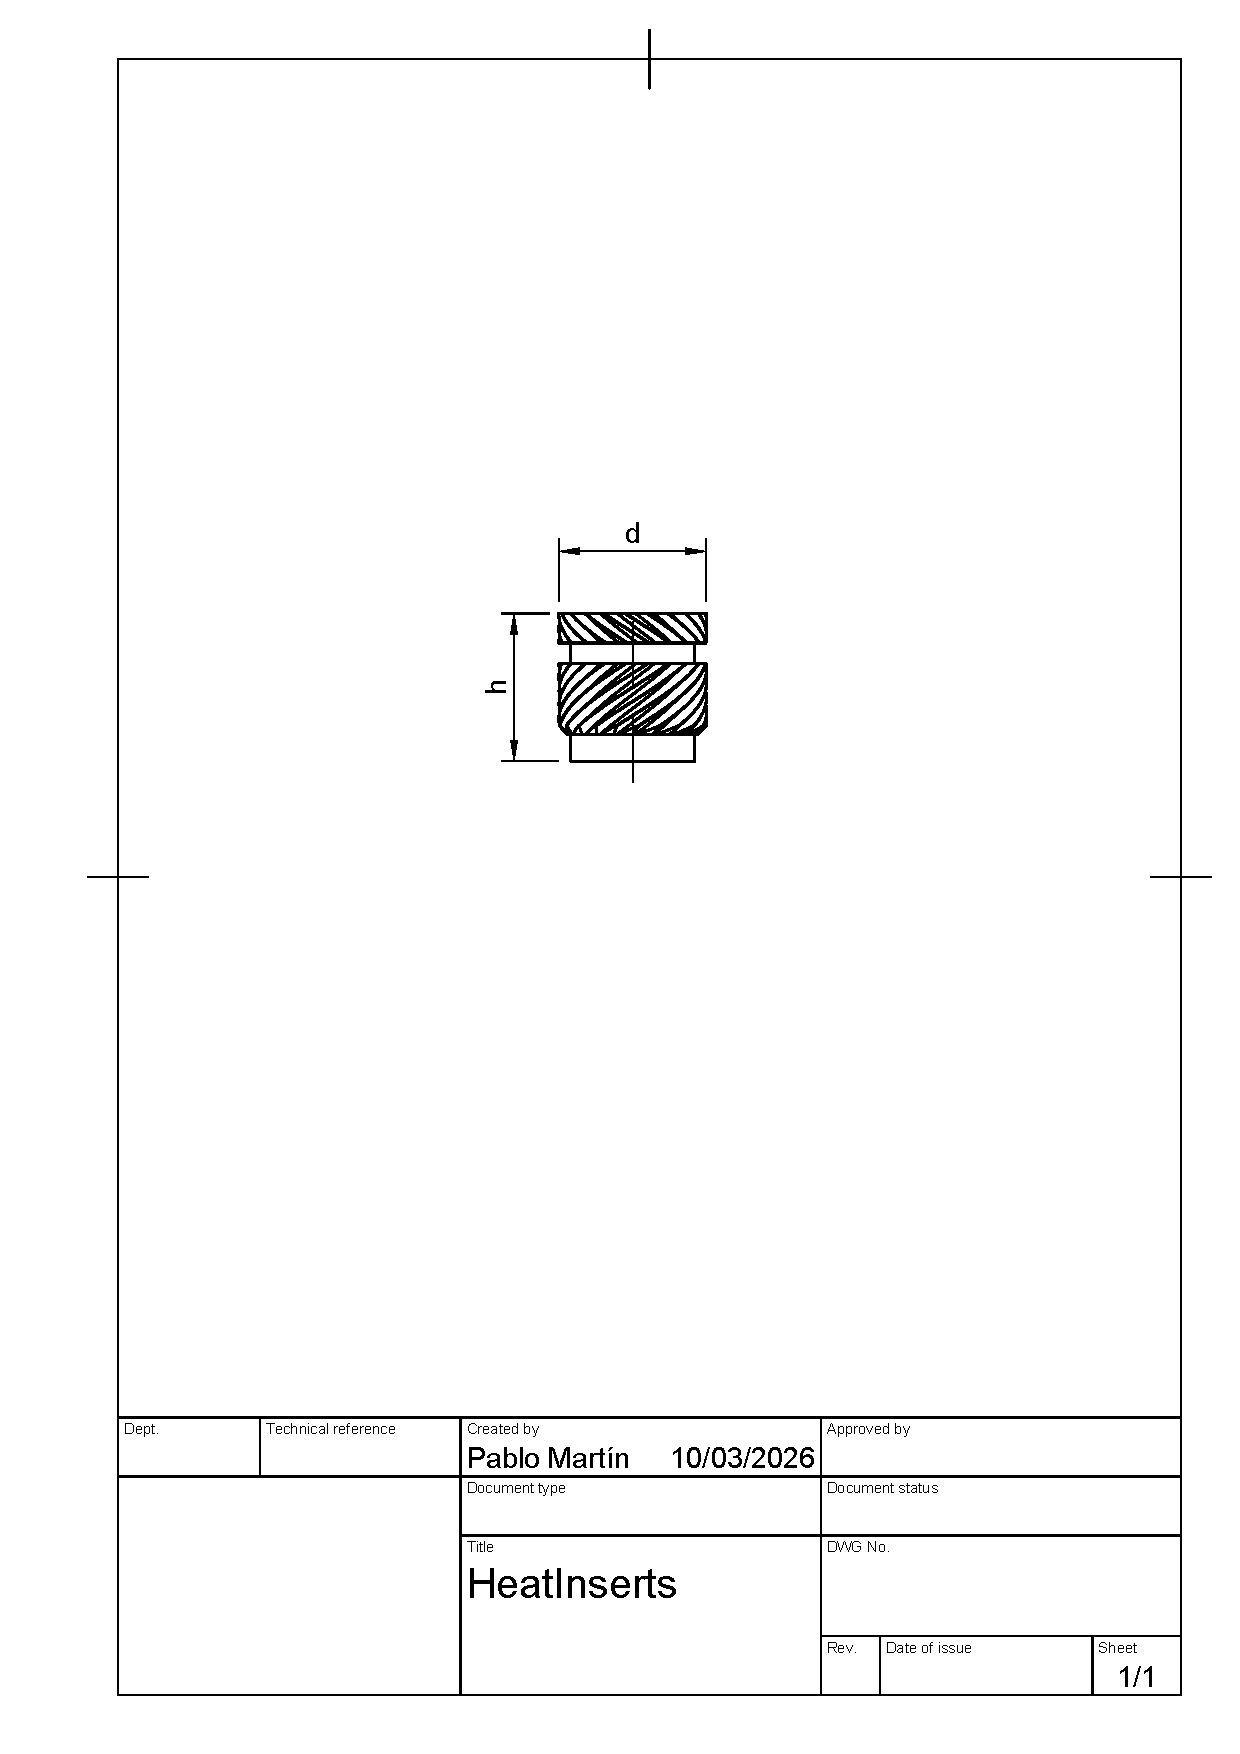
\includegraphics[width=0.5\textwidth, trim={60mm, 160mm, 60mm, 85mm}, clip]{figures/plano-inserto.pdf}
	\caption{Dimensiones relevantes para los insertos roscados}\label{fig:plano-inserto}
\end{figure}

